\documentclass[11pt,a4paper]{article}
\usepackage[utf8]{inputenc}
\usepackage{graphicx}
\usepackage{import}
\usepackage{listings}
\usepackage[english]{babel}
\usepackage{array}

\begin{document}

\begin{figure}[t]
    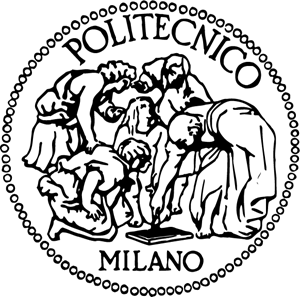
\includegraphics[scale=0.8]{logo_polimi.png}
    \centering
\end{figure}

\begin{titlepage}
    \newcommand{\HRule}{\rule{\linewidth}{0.5mm}}
    \center
    \textsc{\LARGE POLITECNICO DI MILANO}\\[1.5cm]
	
	\textsc{\Large SOFTWARE ENGINEERING II}\\[0.5cm]
	
	\HRule\\[0.4cm]
	    {\huge \textsc{SafeStreets - \\Requirements Analysis and Specification Document}}\\[0.4cm]
	    Version 1.0
    \HRule\\[1.5cm]
	
	\begin{minipage}{1\textwidth}
		\begin{flushleft}
			\large
			\textit{Authors}\\
			Iacopo \textsc{Marri}\\
			Manuel \textsc{Salamino}\\
			Steven Alexander \textsc{Salazar Molina}
		\end{flushleft}
	\end{minipage}
	
	\vfill\vfill\vfill % Position the date 3/4 down the remaining page
	
	{\large\today}
	
\end{titlepage}


\newpage

\tableofcontents

\section{Introduction}
The Requirement Analysis and Specification Document (RASD) aims to focus on the tasks needed to develop and implement an application, taking account of the requirements of the involved stakeholders and, analyzing and documenting also the application requirements.\\
Then, in the second part of the document, there is a more formal definition of the requirements with the use of the Alloy language.\\
In general this document is meant for developers tasked with the implementation of the System and also for all the other entities involved in validation and managing of the project.

\subsection{Purpose}
\textit{SafeStreets} is an application that was created with the intention of monitoring the compliance with traffic regulations. Its goal is to allow Users to notify traffic violations, collect those data about them, elaborate into information, and then provide them to both Users or authorities who need, for aiming different scopes. \\ \\
The application provides Users a way to send data about a violation (most common are parking violations ones, e.g. vehicles parked in reserved places), like the kind of violation, pictures of the involved vehicles, and the date and the position in which the violation occurred. The User can also specify the license plate of the vehicle and the name of the street, but in case he/she doesn't, the application is equipped with algorithms capable to obtain those and other metadata by pictures and position.\\\\
SafeStreets stores all these data, received ones and computed ones, and allows Users and competent authorities to access them, in order to gather useful information about traffic and violations, e.g. areas with the higher number of violations. This could, for example, help municipality to identify areas in which they must watch over.\\\\
Moreover, the System is also able to combine its own data, with data provided by municipality authorities, in case they offer a service that provides them. Basing on the information obtained in this way, SafeStreets will give suggestions about how to improve urban mobility situation, or about how to prevent some kind of violations from being committed (e.g. putting some cameras in vulnerable areas, add some kind of barrier and so on).\\\\
For last, authorities are allowed to use information provided by the application and generate traffic tickets. This leads the application to having to implement a method for ensuring the integrity of the incriminating data, from when the data is generated, to when it is delivered to the application. authorities have to be sure, for example, that they're not giving a fine to a vehicle just because of a picture alteration has been carried out by a notifying User, so altered information must be discarded. SafeStreets will also use statistics on those "rotten" data with the aim to do measure on number of bad Users, or to monitor the reliability and effectiveness of the application it self. \\\\

Here below are listed out the goals we did talk about:

\begin{itemize}
\item {[G.1]} Allows the User to access the functionalities of the application from different locations and devices.
\item {[G.2]} Allows the User to notify about traffic violations.
\item {[G.3]} Allows the User to send pictures and kind of the violation, and other information like the license plates of involved vehicles.
\item {[G.4]} Must attach other metadata to the data sent by the User.
\item {[G.5]} Must be able to obtain data like the license plates, or the name of the street involved in the violation, by the pictures and the position sent by the User.
\item {[G.6]} Must store all of these information in a secure way.
\item {[G.7]} Allows both normal Users and authority Users to access its data, and gather relevant information about streets and violations (e.g. streets with more violations).
\item {[G.8]} Must cross its data with the municipality ones, if they provide an interface for allowing other users to access them.
\item {[G.9]} Must provide suggestions to improve traffic safety.
\item {[G.10]} Must ensure that if any corrupted information is provided by Users, it get discarded.
\item {[G.11]} Must use altered data to provide statistic analysis.
\item {[G.12]} Allows Users with authority permissions to generate traffic tickets from its information.   


\end{itemize}

\subsection{Scope}
    According to the World and Machine paradigm, introduced by M. Jackson and P. Zave in 1995. We can idenfity the Machine as the System to be developed and the environment in which SafeStreets will be used as the World. The separation between these two concepts allow us to classify the entire phenomena in three different types.
    \vspace{0.5cm}
    
    % to be fixed vspace
    
    \noindent\textbf{World phenomena}, events that take place in the real world and that the machine cannot observe.
    \begin{itemize}
      \item The driver has an accident and leaves the car in an inappropriate place.
      \item A malicious user reports a fake traffic violation.
      \item A user has an old mobile phone with a low quality camera.
      \item Movement of a user from a position to another one before sending the picture.
      \item Unexpected connection losses before receiving a picture.
    \end{itemize}
    \vspace{0.5cm}
    
    \noindent\textbf{Machine phenomena}, events that take place inside the \textit{System} and cannot be observed by the real world.
    \begin{itemize}
      \item Encryption of sensitive data.
      \item All operations performed to store/retrieve collected data.
      \item The System retrieves information about unsafe areas from municipalities' services.
      \item The System manages multiple reports of the same traffic violation.
    \end{itemize}
    \vspace{0.5cm}
    
    \noindent\textbf{Shared phenomena:}\\\newline
    Controlled by the world and observed by the machine.
    \begin{itemize}
      \item A guest can sign up to the application or log in if is already registered.
      \item The User can send report traffic violations at any time.
     % levato questo perché forse non ha senso 
     % \item The User can add further information in order to help authorities in the identification of the car's owner.
      \item The Municipality offers up-to-date information about accidents on the territory.
    \end{itemize}
    
    \noindent{Controlled by the machine and observed by the World.}
    \begin{itemize}
      \item The System sends traffic violations to authorities.
      \item The System allows users to view own reports.
      %forse no?
      %\item The \textit{System} asks and verifies the identity of the User.
      \item The System shows inferred safe/unsafe areas.
      \item The Municipality gets suggestions generated by the System.
      \item The System allows authorities to generate traffic tickets
      \item The System notifies authorities about adulterated pictures. 
      \item The User can view  statistics built by the System.
      % (non mi piace tantissimo la parola view, se avete qualche altra parola in mente fatemi  sapere)
    \end{itemize}

\subsection{Definitions, Acronyms, Abbreviations}
    \subsubsection{Definitions}
        \begin{itemize}
            \item \textbf{Guest}: a person who 
            \item \textbf{User}: a person that uses the application to send notifications of traffic violations.
            %forse employee era meglio?
            \item \textbf{Authority}: a municipality worker that is able to create traffic tickets depending on the violation that a person has committed.
            \item \textbf{Data provided by Municipality}: all the information about traffic tickets generated in past and traffic tickets that are generated by using SafeStreets.
            \item \textbf{Sensitive data}: any kind of information that could be used to identify the User who reported a traffic violation.
            %forse areas that may be dangerous to Users, era meglio?
            \item \textbf{Unsafe areas}: areas in which a high number of traffic violations took place.
            \item \textbf{Statistics}: information that allows to show particular queries to the database, for example it is possible to ask the DBMS for the offender who has committed the highest number of violations, the safest area, the number of tickets that are being generated and so on.
        \end{itemize}
        
    \subsubsection{Acronyms}
    \begin{itemize}
        \item DBMS: Data Base Management System
        \item UI: User Interface
        \item API: Application User Interface
    \end{itemize}
    \subsubsection{Abbreviations}
        \begin{itemize}
            \item {[\textbf{G.i}]} : i-th goal.
            \item {[\textbf{D.i}]} : i-th domain assumption.
            \item {[\textbf{R.i}]}: i-th functional requirement.
            \item {[\textbf{R.i-NF}]}: i-th non functional requirement.
            \item {[\textbf{UC.i}]}: i-th use case.
        \end{itemize}
    

\subsection{Revision
history}

\subsection{Reference
Documents}
    \begin{itemize}
        \item Alloy Documentation
        \item Project assignment specifications
    \end{itemize}

\subsection{Document
Structure}

\textbf{Section 1} introduces the problem and describes the purpose of the application SafeStreets. Furthermore, describes the scope in which the application is defined by stating the goals and a brief description of phenomena.\\\\
\textbf{Section 2} presents the overall description of the project. \textit{Product Perspective} give more details about the boundaries of the system and world, machine and shared phenomena, while in \textit{Product Functions} are described the main functions of the system and in \textit{User Characteristics} the main actors. At last are defined the domain assumption on which the system relies on.\\\\
\textbf{Section 3} contains all the specific requirements needed to satisfy each goal. Furthermore, are highlighted the major functions and interactions between the actors and the system using use cases and sequence diagrams.\\\\
\textbf{Section 4} shows the alloy model and discuss its purpose.\\\\
\textbf{Section 5} explain the effort spent by each group member to accomplish this project.\\
\section{Overall Description}

% mettere in automatico Section [number]
\subsection{Product
perspective}
Here we discuss in details all the shared phenomena outlined in Section 1.3 and we also provide a domain model through class and state diagrams.
\\\newline
    \noindent\textbf{Shared Phenomena, controlled by the world and observed by the machine. }
\begin{itemize}
    \item Register/login: a normal person or a municipality worker can register to the application through two different intuitive forms; SafeStreets collects all the information inserted by the User, creates an account and verify the validity of the information given through a email-confirmation message. Once the User confirms its account he/she can proceed to login.
    \item Report of a traffic violation: the User is able to report traffic violations at any time, he/she can open the application, select \textit{take a picture} and then send the report including the picture, the type of violation and the name of the street where the violation occurred.
    %levato perché forse non ha senso
    %\item Addition of further information: the User can add further information to the report that is going to be sent, the information can be the license plate of the car, the exact street in which the car was parked, the time in which
    \item The Municipality offers up-to-date information about accidents: in the Municipality web platform there is a service (daily updated) that indicates streets in which accidents occurred. In this way the System can observe safe/unsafe areas.
\end{itemize}

    \noindent\textbf{Shared Phenomena, controlled by the machine and observed by the world.}
      \begin{itemize}
      % controllare se forwarding va bene
          \item Forwarding of traffic violations: every time a user sends a traffic violation, the System forwards it to the authorities. The message sent by the System contains the photo of the violation, the type of violation, the street in which it took place and the area in which the photo was taken (since there may be more than one street with that name).
          \item Visualization of own reports: the System makes it possible for the users to view the own reports by performing a query to the database and displaying them in a ListView in the application.
          %forse no?
          %\item Verification of identity of the User:
          \item Visualization safe/unsafe areas: the System through the service offered by the municipality is able to get a list of areas in which accidents took place, thus the System can show unsafe and safe areas to the User.
          % c'è una parola per una cosa che avviene spesso, ma non me la ricordo, se ve la ricordate fatemi sapere per favore. grazies.
          \item Suggest possible interventions: the System,  by using a list of known and effective solutions for some common violations, is able to suggest possible interventions in order to reduce the number of violations and make unsafe areas safer.
          % poi safer non mi piace tantissimo
          \item Generate traffic tickets: the municipality, by observing the reports provided by Safe4Streets, is able to  generate traffic tickets by using a functionality of the application.
          % forse non ci va funcionality ma opzione
          \item Notify about modified photos: if the User modifies a photo in order to send malicious reports, the system mark the User as a malicious User and sends a message about this event to authorities (that already received reports created by the User). 
          % mi ricordavo che to illustrate è bello da dire
          \item Generate statistics: the System is able to generate graphs that illustrate statistics, like the most egregious offenders, the effectiveness of the application itself, etc.
          \end{itemize}
          
      


\subsection{Product
functions}

\textbf{SafeStreets}\\

\textit{SafeStreets} was born with the intention of improving urban traffic mobility, by collecting notifies made by Users about many kinds of traffic violations. Then these information can be consulted by Users themselves, or from a Third Part, the traffic competent authorities, or the municipality, which can create tickets based on these information, on which integrity it is necessary to pay particular attention. Indeed, \textit{SafeStreets} provides useful suggestions built upon the crossing of municipality's and \textit{SafeStreets}'s data. \\
Let's see more in the details the functions mentioned above:\\\\

\textbf{Basic User functions} \\
\begin{itemize}
    \item \textbf{Notifying violations}\\\\
    The Users who is witness of a rule violation, and wants to notify it through \textit{SafeStreets}, has to be registered to the application; then he/she can fill up the notification form provided by the application, with a picture or a video of the violation occurring, the kind of violation, the kind of vehicle, the position, (or the address, which can be anyway gathered from GPS), and the license plate of the indeed vehicles.\\
    Not all of these data are mandatory for the User to send, only a picture, the GPS position and the kind of violations are: \textit{SafeStreets} uses an algorithm to catch the license plates from the picture, can obtain the address by the GPS position, and it implements a deep learning algorithm to recognize the vehicles by it self. \textit{SafeStreets} is going to attach these computed metadata to the notification, in case of missing. Time is automatically taken from the notification delivery time.
    
    \item\textbf{Mining information from data}\\\\
    Registered Users (quelli non registrati possono?) can access the  data stored by the application, in order to mine useful information. \\ \textit{SafeStreets} provides an easy-use interface that allows to  carry out a search for violations based upon different criteria: the \textit{kind} of the violations, the \textit{place} in which happen, the \textit{time}, and the \textit{kind of vehicle} involved. 
    A user can then extract information from this data, for example, search for a place, and than see at which time slot of the day, more violations are committed in that place, or in which place or at which time slot, a precise type of violation occurs the most.\\
    By the way, due to privacy purposes, license plates related to violations are not visible by a normal User, neither a User can search some information about a precise vehicle with a precise license place.
    
    \end{itemize}  
    
    \textbf{Authority Users functions} \\
    
    \begin{itemize}
   
    
    \item\textbf{SafeStreets suggestion mechanism}\\\\
    If the local municipality provides a way to access their own urban traffic and violations data, \textit{SafeStreets} can cross them, to enlarge the amount of information accessible, and exploit them to formulate suggestions for the municipality, in order to increase the functionality of the urban infrastructure, reduce the violations, improve road conditions.\\ Authorities and municipality can ask for these suggestions for various areas, with a function button on the application interface.\\
    Imagine a situation in which \textit{SafeStreets} knows about huge amount of bike lane invasion violations, and municipality knows that in that zone, many people use bikes for moving, then \textit{SafeStreets} can cross those information and provide the suggestion to build a separation line between the car road, and the bike lane, because it should be a good investment, knowing the fact that not only there are lots of violations, but also that those could be very dangerous, given the number of people using bike in that zone. 
    
    
     
    \item\textbf{Searching for violations}\\\\
    In addition to the mining functions provided for normal users, Authorities can also access some more "sensible data", and carry out more precise searches about violations. They can access the list of violations, with relatives license plates and data of involved people. In order to build this authorization diversification, a different type of registration will be reserved for authorities Users. (Da decidere come).
    Authorities can also use the application to get suggestions about which are the most unsafe urban areas, and how to get them better.
    
    
    \item\textbf{Traffic tickets service}\\\\
    \textit{SafeStreets} give road Authorities the possibility to generates traffic tickets from the violations information sent by Users. An appointee authority User can check a notified violation and all the data attached to it, confirm that it is actually a violation, and then the use function provided by \textit{SafeStreets} (that is linked to the authorities management system) to generate a ticket. \\
    In order to make this right, \textit{SafeStreets} has to ensure that the chain of custody of the data, from the user to the data store, is completely reliable. To do this, security algorithms perform a validity check on the sent pictures, to be sure the picture is not been modified. In case it is, discard the notification. Discarded data are used to make statistical analysis.
    Another filtering level is applied by allowing Users to only send pictures taken while filling up the notification form, and not to upload previously taken ones. In this way, it's harder for a User to modify a picture before sending it. 
\end{itemize}

\subsection{User
characteristics}
% se non vi piace possesses pssiamo cambiarlo
SafeStreets is an application suitable for any adult person that possesses a mobile phone.
\subsubsection{Actors}
\begin{itemize}
    \item \textbf{Guest}: a person who downloaded the application and still has to register, he cannot use any functionality of the application.
    \item \textbf{User}: once a guest has registered through the initial form of the application, he gets an account with a \textit{username} and a \textit{password}. Moreover, the User has accepted to give his location and access to the camera of the mobile phone.
    \item \textbf{Authority}: a municipality worker that is able to generate traffic tickets from the violations reported. Furthermore, he can access to other functionalities that a simple user cannot even see.
    %non mi viene in mente nessun altro
    %\item \textbf{}
\end{itemize}
\subsection{Assumptions,
dependencies
and
constraints}
\subsubsection{Domain Assumptions}
\subsubsection{Dependencies}
\subsubsection{Constraints}

\section{Specific Requirement}

\subsection{External Interface Requirements}

\subsubsection{User Interfaces}

\subsubsection{Hardware Interfaces}

\subsubsection{Software Interfaces}

\subsubsection{Communication Interfaces}

\subsection{Functional Requirements}

    \subsubsection{Sequence Diagrams}
    
    \begin{figure}[h]
        \centering
        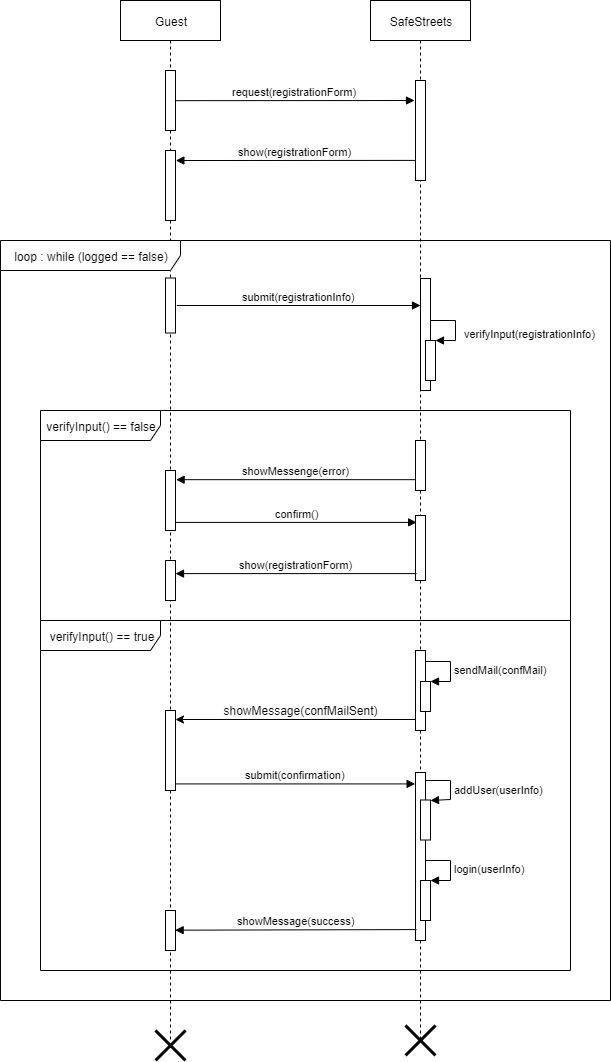
\includegraphics[scale=0.5]{SeqDiag_registration.png}
        \caption{Sequence Diagram of the registration of a User}
    \end{figure}
    
    \begin{figure}[h]
        \centering
        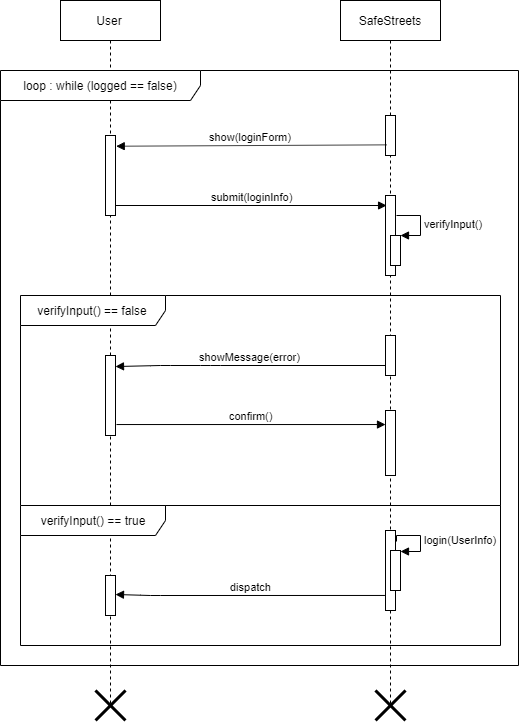
\includegraphics[scale=0.5]{SeqDiag_login.png}
        \caption{Sequence Diagram of the login of a User or of an Authority}
    \end{figure}
    
    \begin{figure}[h]
        \centering
        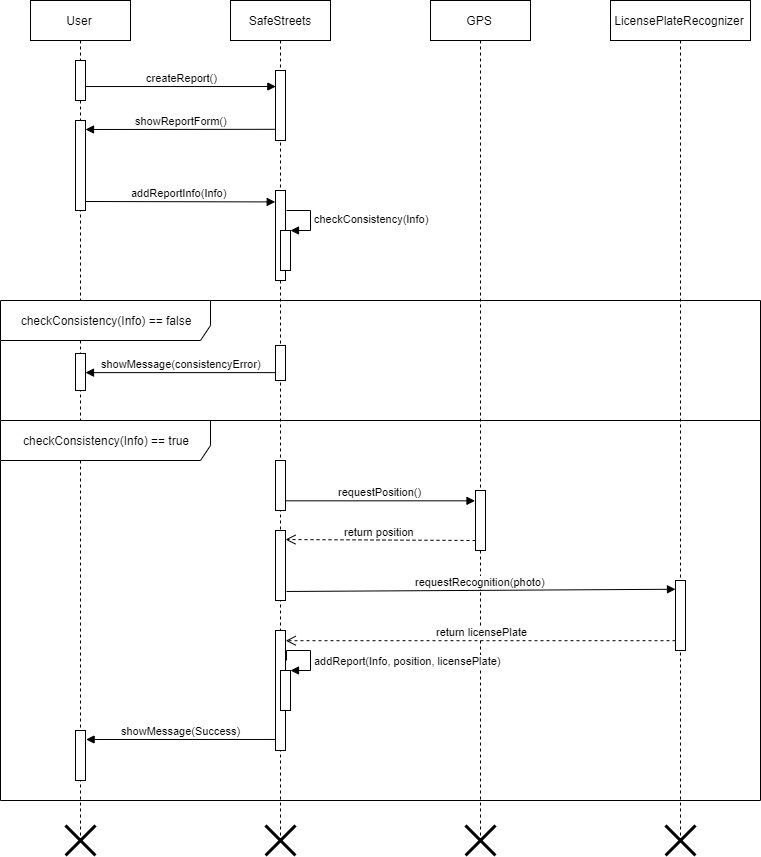
\includegraphics[scale=0.5]{SeqDiag_addReport.png}
        \caption{Sequence Diagram of the insertion of a Report by a User}
    \end{figure}
    
    \begin{figure}[h]
        \centering
        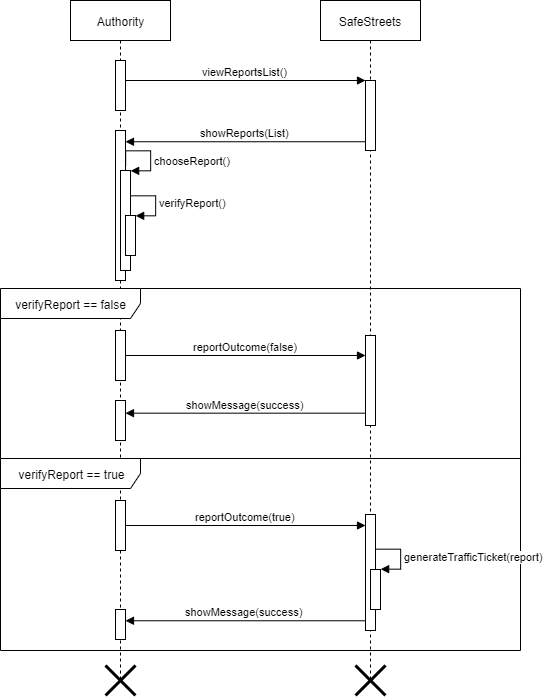
\includegraphics[scale=0.5]{SeqDiag_generateTrafficTicket.png}
        \caption{Sequence Diagram of the checking of a Report and, eventually, the generation of the corresponding Traffic Ticket}
    \end{figure}
    
    \begin{figure}[h]
        \centering
        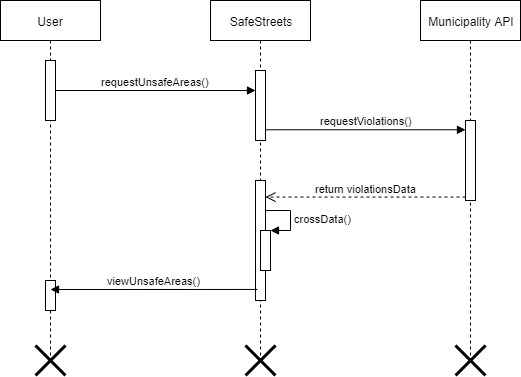
\includegraphics[scale=0.5]{SeqDiag_unsafeAreas.png}
        \caption{Sequence Diagram of the request to know which are the unsafe areas}
   \end{figure}

\subsection{Performance Requirements}

\subsection{Design
Constraints}

\subsubsection{Standards compliance}

\subsubsection{Hardware
limitations}

\subsubsection{Any other constraint}

\subsection{Software System Attributes}

\subsubsection{Reliability}

\subsubsection{Availability}

\subsubsection{Security}

\subsubsection{Maintainability}

\subsubsection{Portability}
\section{Formal Analysis using Alloy}
\section{Effort Spent}
The following tables summarize the effort spent by each member of the team to create the RASD document.
\subsection{Marri Iacopo}
% forse era meglio 'time' al posto di effort?
\begin{center}
% crea un po' di margine tra il testo e i bordi della tabella
\renewcommand{\arraystretch}{1.5}
\begin{tabular}{ |m{7cm}|m{2cm}| } 
 \hline
 \textbf{Description of the task}  & \textbf{Hours} \\
 \hline
 First meeting + Github setup & 4 \\
 \hline
 Purpose, Scope and Definition & 5 \\
 \hline
 Product Perspective & 5 \\ 
 \hline
 Product Functions & 2 \\ 
 \hline 
 User Characteristics and Assumptions, dependencies and constrains & 2.5 \\ 
 \hline
 Specific Requirement & 3 \\
 \hline
 Alloy & \\
 \hline
\end{tabular}
\end{center}


\subsection{Salamino Manuel}
\renewcommand{\arraystretch}{1.5}

\begin{center}
\begin{tabular}{ |m{7cm}|m{2cm}| } 
 \hline
 \textbf{Description of the task}  & \textbf{Hours} \\
 \hline
 First meeting + Github setup & 4\\
 \hline
 Purpose, Scope and Definition & 6 \\
 \hline
 Product Perspective & 8 \\ 
 \hline
 Product Functions & 2 \\ 
 \hline 
 User Characteristics and Assumptions, dependencies and constrains & 2 \\ 
 \hline
 Specific Requirement & 4 \\
 \hline
 Alloy & \\
 \hline
\end{tabular}
\end{center}

\subsection{Salazar Molina Steven Alexander}
\begin{center}
\renewcommand{\arraystretch}{1.5}

\begin{tabular}{ |m{7cm}|m{2cm}| } 
 \hline
 \textbf{Description of the task}  & \textbf{Hours} \\
 \hline
 First meeting + Github setup & 4 \\
 \hline
 Purpose, Scope and Definition & 5.5 \\
 \hline
 Product Perspective & 5 \\ 
 \hline
 Product Functions & 4 \\ 
 \hline 
 User Characteristics and Assumptions, dependencies and constrains & 4.5 \\  
 \hline
 Specific Requirement & 5 \\
 \hline
 Alloy & \\
 \hline
\end{tabular}
\end{center}

% ho tolto References perché ho notato che Diego/loris, lo scarlatti, giò e negri non avevano questo sezione. ho letto il loro assigment ed era come il nostro (indicato References come sezione 6) ma non l'hanno fatto quindi boh, lo chiederei al prof nel caso perché c'è anche una sottosezione nella sezione 1 in cui chiede 'document references'
%\section{References}

\end{document}
